\subsection{Aufbau des Touchscreen GUI's}
	Nun also zur Software. 
	Das System ist als Event gesteuertes UI in seinen Grundzügen stark \texttt{Java Swing} angelehnt.
	Die implementierten Komponenten sind typische Kontrollen eines Touch GUI.
	Kern des Systems ist eine Abstraktion des Touchscreens auf dem Daughterboard.
	
	\subsubsection{Die Klasse TouchScreen}\label{sec:touchscreen_class}
		\begin{wrapfigure}[14]{R}{0.4\textwidth}
			\scalebox{0.75}{
				\begin{tikzpicture}
					\begin{class}[text width=7.5cm]{TouchScreen}{0, 0}
	\attribute{- x, y: WORD}
	\attribute{- touchCount: WORD}
	\attribute{- width, height: WORD}
	\attribute{- i2cTouch: cHwI2Cmaster::Device\&}
	\attribute{- interruptPort: cHwPort\_N::PortId}
	\attribute{+ interruptPin: BYTE}
	\attribute{+ rootContainer: Container*}
	\attribute{+ \emph{static} INSTANCE: TouchScreen*}
	
	\operation{+ refresh(): void}
	\operation{+ setInterruptMode(mode: bool): void}
	\operation{+ interruptHandler(): void}
	\operation{+ setRootContainer(c: Container*): void}
	\operation{+ getRootContainer(): Container*}
\end{class}
				\end{tikzpicture}
			}
			\caption{Klassendiagramm TouchScreen}
			\label{uml-touchscreen}
		\end{wrapfigure}
		Diese Klasse (\ref{uml-touchscreen}) bietet verschiedene Methoden, welche die Kommunikation mit dem Daughterboard umsetzen und ist als \emph{Singelton} entworfen.
		Die statische Variable \texttt{INSTANCE} speichert die (einzige) Instanz dieser Klasse, um ihren \texttt{InterruptHandler} aus \texttt{linkage "C"} aufrufen zu können.
		
		Um das System nicht unnötig auszulasten, ist die Instanz in der Lage, einen GPIO-Interrupt zu behandeln.
		Das Daughterboard ist in der Lage eine erkannte Berührung durch das auf \texttt{LOW} ziehen der \texttt{INT} Leitung zu signalisieren \cite[8\psq]{ts-userManual}.
		Diese Leitung ist über den Stecker \texttt{CN1} auf Pin 4 mit dem Motherboard verbunden. Dieser entspricht dem Pin \texttt{PI13} des $\mu C$ \cite[27\psq]{disco-userManual}.
		
		Der \texttt{EXTI} Controller des $\mu C$ ist für das Erzeugen eines Interrupts, beim Eintreten eines Signals auf einer Input Line (einem Pin des $\mu C$), zuständig.
		Der \texttt{EXTI} Controller ermöglicht das Maskieren einzelner Interrupts und Selektion der Flanke des Signals, die den Interrupt auslösen soll. \cite[319\psqq]{stm32_refManual}
		
		Ein ausstehender Interrupt, konfiguriert durch den \texttt{EXTI} Controller, wird durch das aufrufen der Interruptroutine durch den \texttt{Nested vectored interrupt controller} (\texttt{NVIC}) behandelt \cite[313\psqq]{stm32_refManual}.
		Der entsprechende Interrupt muss im \texttt{SYSCFG} Register freigeschaltet werden, dies passiert anhand seiner \texttt{IRQNumber}.
		
		Sobald eine Berührung erkannt wird, wird der entsprechende \texttt{IRQHandler} aufgerufen.
		Dieser ruft nun den \texttt{InterruptHandler} der Instanz der \texttt{TouchScreen} Klasse auf.
		Diese fragt dann durch \texttt{refresh()} die aktuellen Daten über den I²C-Bus vom Daughterboard ab und erzeugt ein entsprechendes \secref{EventSystem}{Event}.
		Dieses Event wird schließlich an den \texttt{RootContainer} übergeben, welcher es an seine Komponenten weitergibt.
	
	\subsubsection{Komponenten und Container}\label{sec:components}
		\begin{wrapfigure}[12]{R}{0.4\textwidth}
			\scalebox{0.75}{
				\begin{tikzpicture}
					\begin{abstractclass}[text width=11cm]{Component}{0, 0}
	\attribute{\# box: BoundingBox}
	
	\operation{+ Component(x: WORD, y: WORD, w: WORD, h: WORD)}
	\operation{+ getBoundingBox(): BoundingBox\&}
	\operation[0]{+ onEvent(event: DragEvent\&): void}
	\operation[0]{+ onEvent(event: TouchEvent\&): void}
	\operation[0]{+ onEvent(event: ReleaseEvent\&): void}
	\operation[0]{+ show(display: cDevDispalyGraphic\&): void}
\end{abstractclass}
				\end{tikzpicture}
			}
			\caption{Klassendiagramm Component}
			\label{uml-component}
		\end{wrapfigure}
		Alle Komponenten haben die gemeinsame Oberklasse \texttt{Component} (\ref{uml-component}), welche drei Aspekte der Komponenten modelliert. Erstens: die \texttt{BoundingBox}, ein achsparalleles Rechteck, welches die Komponente vollständig enthält.
		Eine Komponente erhält Touchscreen-Events nur, wenn diese in ihrer \texttt{BoundingBox} liegen.
		Zweitens: drei Methoden, welche Touchscreen-Events annehmen und verarbeiten.
		Drittens: eine Methode, welche die Komponente auf ein Display zeichnen kann.
		
		Einzelne Komponenten können eigene Events auslösen (\texttt{ActionEvents}).
		Diese sind aber komponentenspezifisch und deswegen nicht in der Klasse \texttt{Component} implementiert.
		
		\medskip
		\begin{wrapfigure}[10]{R}{0.4\textwidth}
			\scalebox{0.75}{
				\begin{tikzpicture}
					\begin{abstractclass}{Component}{0, 0}
					\end{abstractclass}
				
					\begin{class}[text width=11cm]{Container}{0, -2.5}
	\inherit{Component}
	
	\attribute{- compontents: list<Component*>}
	
	\operation{+ addComponent(comp: Component*): void}
	\operation{+ removeComponent(comp: Component*): void}
\end{class}
				\end{tikzpicture}
			}
			\caption{Klassendiagramm Container}
			\label{uml-container}
		\end{wrapfigure}
		Ein \texttt{Container} (\ref{uml-container}) dient nur dazu, mehrere Komponenten in einer Gruppe zusammenzufassen.
		Bestände die Möglichkeit, eine Komponente zu \emph{deaktivieren}, wäre es Aufgabe dieser Klasse diese Operation an ihre Komponenten weiterzugeben.
		Beispielsweise könnte eine Gruppe von \texttt{RadioButtons} -- in einem Container zusammengefasst -- durch nur einen Aufruf deaktiviert werden.
		Dieses Feature ist aber nicht implementiert, demnach ist der \texttt{Container} nur eine logische Einheit.
		
		Da ein \texttt{Container} von \texttt{Component} erbt, ergibt sich eine Hierarchie der Komponenten. Ziel dessen ist es, das Interface möglichst modular gestalten zu können.
		
		\medskip
		\begin{wrapfigure}{R}{0.4\textwidth}
			\scalebox{0.75}{
				\begin{tikzpicture}
					\begin{abstractclass}{Component}{-3, 0}
					\end{abstractclass}
				
					\node[right=of Component] (image) {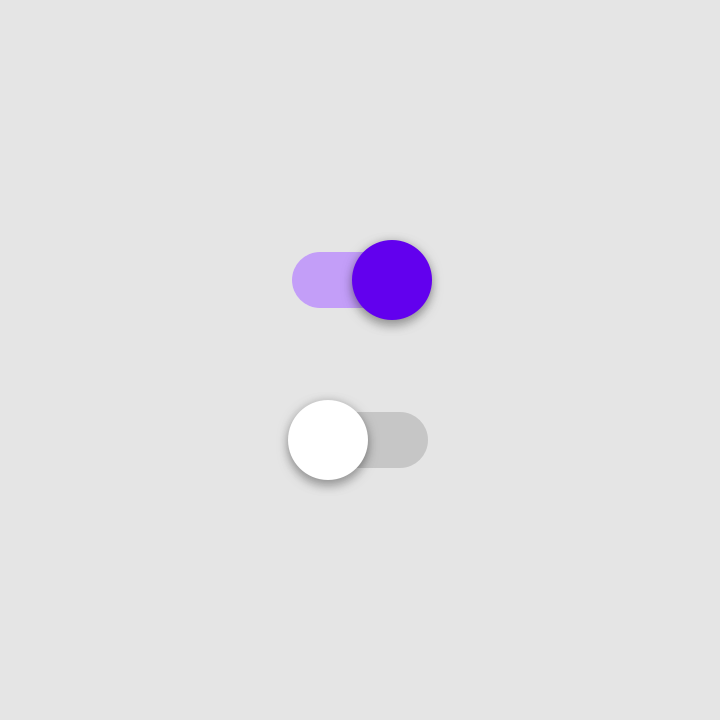
\includegraphics[height=2cm]{../Images/Switch.png}~\cite{material-components}};
					
					\begin{class}[text width=11cm]{ToggleSwitch}{0, -2.5}
	\inherit{Component}
	
	\attribute{- state: bool}
	\attribute{- listeners: list<function<void(ToggleSwitchEvent\&)>\relax>}
	
	\operation{+ getState(): bool}
	\operation{+ addEventListener(listener: function<void(ToggleSwitchEvent\&)>): void}
\end{class}
				\end{tikzpicture}
			}
			\caption{Klassendiagramm ToggleSwitch}
			\label{uml-toggleswitch}
		\end{wrapfigure}
		Ein \texttt{ToggleSwitch} (\ref{uml-toggleswitch}) dient zum Setzen einer Ein/Aus-Einstellung.
		Dementsprechend speichert die Klasse \texttt{ToggleSwitch} den aktuellen Zustand des Schalters in einem \texttt{bool}.
		Erhält ein \texttt{ToggleSwitch} ein \texttt{TouchEvent} wechselt er den Zustand.
		Außerdem erzeugt er ein \texttt{ToggleSwitchEvent} (eine Subklasse von \texttt{ActionEvent}).
		Dieses wird dann an alle über die Methode \texttt{addEventListener} hinzugefügten Funktionen übergeben.
		Ändert sich der Zustand, dann enthält das korrespondierende \texttt{ActionEvent} den neuen Zustand und wird an alle registrierten \texttt{Listener} übergeben.
		
		\medskip
		\begin{wrapfigure}{R}{0.4\textwidth}
			\scalebox{0.75}{
				\begin{tikzpicture}
					\begin{abstractclass}{Component}{-3, 0}
					\end{abstractclass}
					
					\node[right=of Component] (image) {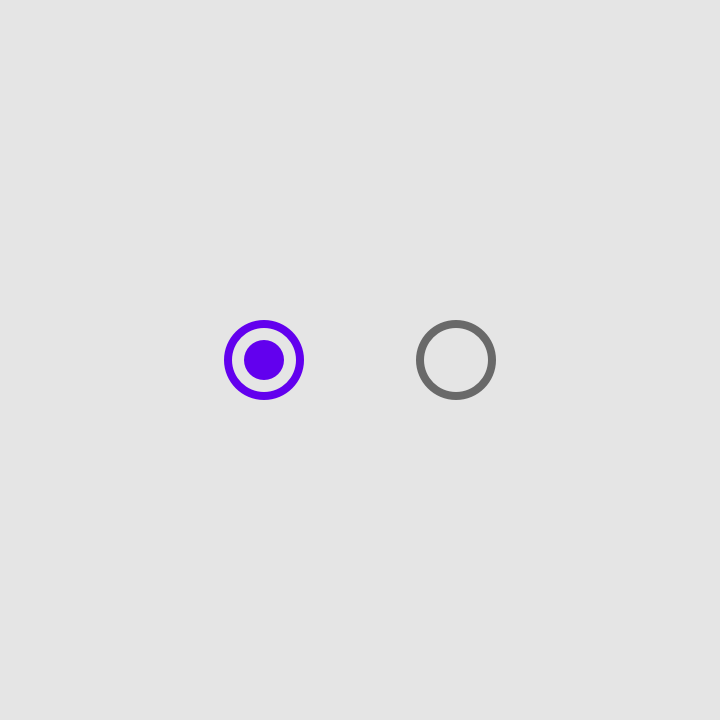
\includegraphics[height=2cm]{../Images/RadioButton.png}~\cite{material-components}};
					
					\begin{class}[text width=11cm]{RadioButton}{0, -2.5}
	\inherit{Component}
	
	\attribute{- state: bool}
	\attribute{- deselectable: bool}
	\attribute{- listeners: list<function<void(RadioButtonEvent\&)>\relax>}
	
	\operation{+ getState(): bool}
	\operation{+ addEventListener(listener: function<void(RadioButtonEvent\&)>): void}
\end{class}
				\end{tikzpicture}
			}
			\caption{Klassendiagramm RadioButton}
			\label{uml-radiobutton}
		\end{wrapfigure}
		Wie ein \texttt{ToggleSwitch} dient ein \texttt{RadioButton} (\ref{uml-radiobutton}) zum Setzen einer Ein/Aus-Einstellung.
		Im Gegensatz zu einem \texttt{ToggleSwitch} kommuniziert ein \texttt{RadioButton} sich gegenseitig ausschließende Optionen.
		Die beiden Klassen ähneln sich daher stark. Der einzige Unterschied liegt darin, dass es möglich ist, das Abwählen eines
		\texttt{RadioButtons} im Konstruktor zu deaktivieren. Ein \texttt{RadioButton} kann dann nur abgewählt werden,
		indem ein anderer Button der selben Gruppe (also eine andere Option) ausgewählt wird.
		
		\medskip
		\begin{wrapfigure}{R}{0.4\textwidth}
			\scalebox{0.75}{
				\begin{tikzpicture}
					\begin{class}[text width=11cm]{RadioButtonGroup}{0, 0}
	\attribute{- buttons: list<RadioButton*>}
	
	\operation{+ buttonEventHandler(event: RadioButtonEvent\&): void}
	\operation{+ addButton(button: RadioButton*): void}
\end{class}

				\end{tikzpicture}
			}
			\label{uml-radiogroup}
			\caption{Klassendiagramm RadioButtonGroup}
		\end{wrapfigure}
		Diese Gruppen von \texttt{RadioButtons} wird durch eine eigene Klasse (\ref{uml-radiogroup}) modelliert.
		Beim Hinzufügen eines \texttt{RadioButton} in die Gruppe registriert sie die \texttt{buttonEventHandler} Methode als \texttt{Listener} im Button.
		Sobald ein \texttt{RadioButton} ein Event auslöst, setzt diese Methode den Zustand aller anderen Buttons auf \texttt{false}.
		
		\medskip
		\begin{wrapfigure}[11]{R}{0.4\textwidth}
			\scalebox{0.75}{
				\begin{tikzpicture}
					\begin{abstractclass}[text width=3cm]{Component}{-4, 0}
					\end{abstractclass}
					
					\node[right=of Component] (image) {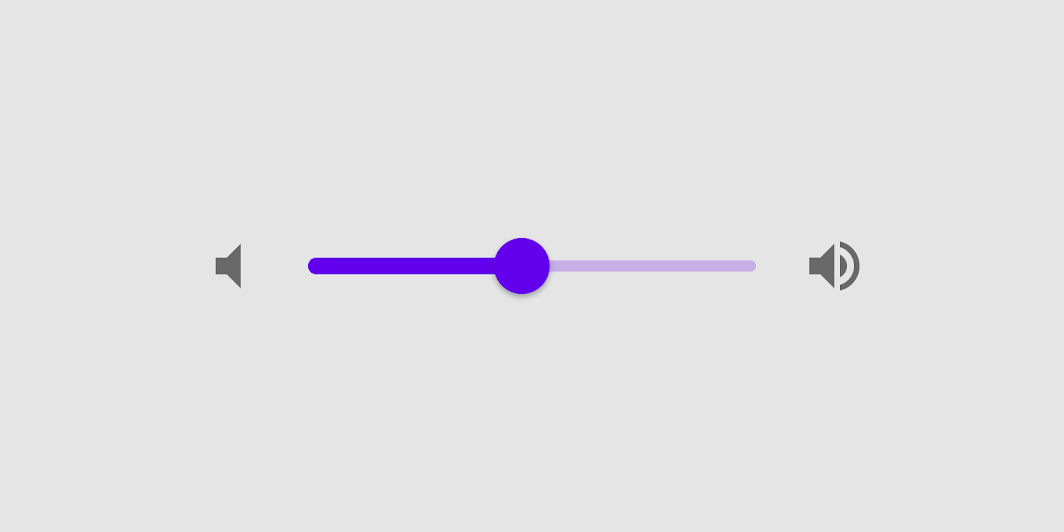
\includegraphics[height=2cm]{../Images/Slider.png}~\cite{material-components}};
					
					\begin{class}[text width=11cm]{Slider}{0, -2.5}
	\inherit{Component}
	
	\attribute{- position: double}
	\attribute{- listeners: list<function<void(SliderEvent\&)>\relax>}
	
	\operation{- setPosition(x: WORD): void}
	\operation{+ getPosition(): double}
	\operation{+ addEventListener(listener: function<void(SliderEvent\&)>): void}
\end{class}
				\end{tikzpicture}
			}
			\caption{Klassendiagramm Slider}
			\label{uml-slider}
		\end{wrapfigure}
		Ein \texttt{Slider} (\ref{uml-slider}) ermöglicht das Auswählen eines Fließkommawertes.
		Das Attribut \texttt{position} speichert die relative Position des \texttt{Sliders} von 0 bis 1.
		Erhält der \texttt{Slider} ein \texttt{TouchEvent}, wird die neue Position bestimmt.
		Die Methode \texttt{setPosition} berechnet den Abstand der Berührung vom Anfang des Bewegungsraumes des \texttt{Sliders}
		und Teilt diesen Abstand durch die Breite des Bewegungsraumes. Anschließend wird $pos \in [0; 1]$ erzwungen.
		
	\subsubsection{Event System}\label{sec:EventSystem}
		Das wichtigste Werkzeug im Entwurf dieses Touch GUI's ist das Event System.
		Ein \texttt{Event} beschreibt eine Berührung oder eine Interaktion des Nutzers mit einem Objekt.
		\texttt{Events} sind aufgeteilt in \texttt{TouchScreenEvents} und \texttt{ActionEvents}.

		\texttt{TouchScreenEvents} werden vom TouchScreen in dessen \texttt{InterruptHandler} generiert und stellen eine einzelne Berührung oder Bewegung dar.
		Sie werden von den in der Hierarchie des Systems eingebetteten Komponenten durch die in \texttt{Component} deklarierten Methoden behandelt
		und bei Bedarf in \texttt{ActionEvents} übersetzt.
		Diese Art Event dient nicht der Umsetzung von Anwendungslogik, sondern ausschließlich der Übertragung von Berührungsdaten an die Komponenten.
		
		\texttt{ActionEvents} werden von einzelnen Elementen des GUI erzeugt und stellen eine Veränderung in deren Zustand dar.
		Sobald eine Komponente eine Änderung ihres Zustandes kommunizieren möchte, kann sie ein entsprechendes \texttt{ActionEvent} erzeugen
		und an ihre registrierten Listener Übergeben.
		
		